\documentclass{article}

\title{Assignment Computer CZ4003 \\ Lab 2}
\date{2019 \\ November}
\author{Koch Philipp Frederik Edward, N1903454H}

\linespread{1.5}

\usepackage{graphicx}
\usepackage{listings}
\usepackage{color}


\definecolor{orange}{rgb}{0.9531,0.39, 0.14}
\definecolor{gray}{rgb}{0.5,0.5,0.5}
\definecolor{green}{rgb}{0,0.6,0}

\lstset{
	basicstyle=\tiny,
	language=Prolog,
	numbers=left,
	numberstyle=\tiny\color{gray},
	keywordstyle=\color{blue},
	commentstyle=\color{orange},
	stringstyle=\color{green},
	lineskip={-1.5pt},
	breaklines=true,
	breakatwhitespace=true,
	frame=single
}

\begin{document}
	
	\maketitle
	
	\section{Edge Detection}

	At first, the sobel mask was created, to transform the picture and make the lines more visible.
	By applying the horizontal filter, the lines became visible in their horizontal position.
	The same applied to the vertical filter with vertical lines.This is due to the sum over the matrix, 
	since the respective axis is always taken into account here.In this application, 
	diagonal edges are crossed on the horizontal or vertical side, so that several parallel lines can be seen here.
	\subsection{Squaring the filtered Images}
	With this method, the areas in the image which are not zero become much larger. This also increases the differences in between the image.
	Thus a clear distinction to the sky becomes clear, since here the gradients in this area of the picture are very small. 
	This method makes the differences between the edges clearer.
	\subsection{Thresholding}
	An operation is now applied to the already squared image, whereby only values above a threshold are being not zero. 
	For the selection of the threshold, a value should be used that is neither too large nor too small. 
	If the value is too small, only areas are separated. If the value is too high, many edges are no longer recognized as such.
	\subsection{Canny Algorithm}
	\subsubsection{Changing the sigma value}
	By a higher sigma, the edges of the distribution fall more strongly in weight. This causes the edges of the distribution to become weaker. 
	The higher the sigma, the fewer corners are detected and only the strong corners are detected. By a stronger approximation, 
	however, also the noises in the picture are removed more strongly. For this aspect, a higher sigma makes sense.
	\subsubsection{Changing the lower threshold}If the lower barrier is changed downwards, more corners are identified as such. 
	If the barrier is raised, these weaker corners are no longer detected.
	Since the Canny algorithm requires a lower limit, this value has a significant effect on the outcome.

	\section{Line Finding using Hough Transform}

	The Hough transformation is discrete, while the Radon transformation is continuous. 
	Since in this case the image is discrete, the radon transformation can be applied here equivalently. After the maximum has been determined, the constant for the lines must now be calculated.
	Since, with the exception of the cases theta = 0° and theta = 180° , a constant exists on the y-axis, this is determined first.
	Since C is unknown and only A and B are known, the line representation y = mx +c must first be used. 
	From the Radon Domain a point can be taken, which represents a line. 
	This line is orthogonal to the searched line, so that the gradient can be determined. 
	To do this, the slope is inverted and the sign is changed. From this representation, the standart form of a line can be easily obtained.
	Now the points yl and yr can be calculated by calculating the intersection points on the y-axis.
	The special case that there is no intersection point on the y-axis was also taken into account.


	\section{3D Stereo}

	\subsection{a)} 
	By using the \textit{conv2} and \textit{rot90} functions, for loops could largely be dispensed with. 
	
	\lstinputlisting[title=Core of the dispfunc Function, firstline=34, lastline=49]{dispfunc.m}
	
	\subsection{b) \& c)}
	Figure 1 shows the distance in the corridor in color. It becomes darker as the distance increases. 
	The intensity in the dispersion map increases as the distance between the similar sections increases with distance. This also increases the distance between the optimal SSD values and therefore the distant surface appears darker.Figure 2 shows the view before the calculation.
	\begin{figure}
		\center
		\caption{Disparity map of the corridor}
		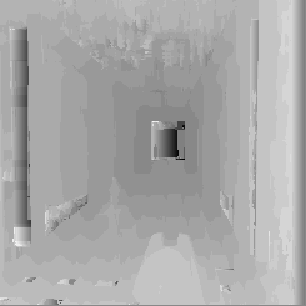
\includegraphics{corridor_disp.png}
		
	\end{figure}
	\begin{figure}
		\center
		\caption{Stereo view before the calculation}
		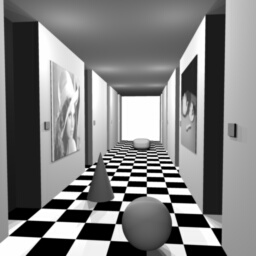
\includegraphics[scale=0.4]{corridorl.jpg}
		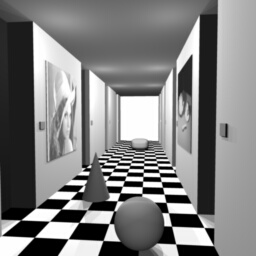
\includegraphics[scale=0.4]{corridorr.jpg}
	\end{figure}
	
	
\end{document}